\documentclass[tikz,border=12pt]{standalone}
\usepackage[T1]{fontenc}
\usepackage{mathpazo}
\usepackage{amsmath,amssymb}
\usetikzlibrary{arrows.meta, positioning, calc, fit, decorations.pathreplacing}
\usepackage{pgfplots}
\pgfplotsset{compat=1.18}

\definecolor{stblue}{HTML}{7B97AD}
\definecolor{rwgold}{HTML}{B8995E}
\definecolor{sage}{HTML}{7A9A7E}
\definecolor{dkbrown}{HTML}{3D3530}
\definecolor{wmgray}{HTML}{7B7067}
\definecolor{cream}{HTML}{F9F6F0}
\definecolor{border}{HTML}{D4C9B8}
\definecolor{terracotta}{HTML}{C47A6A}
\definecolor{lavender}{HTML}{907EA0}

\begin{document}
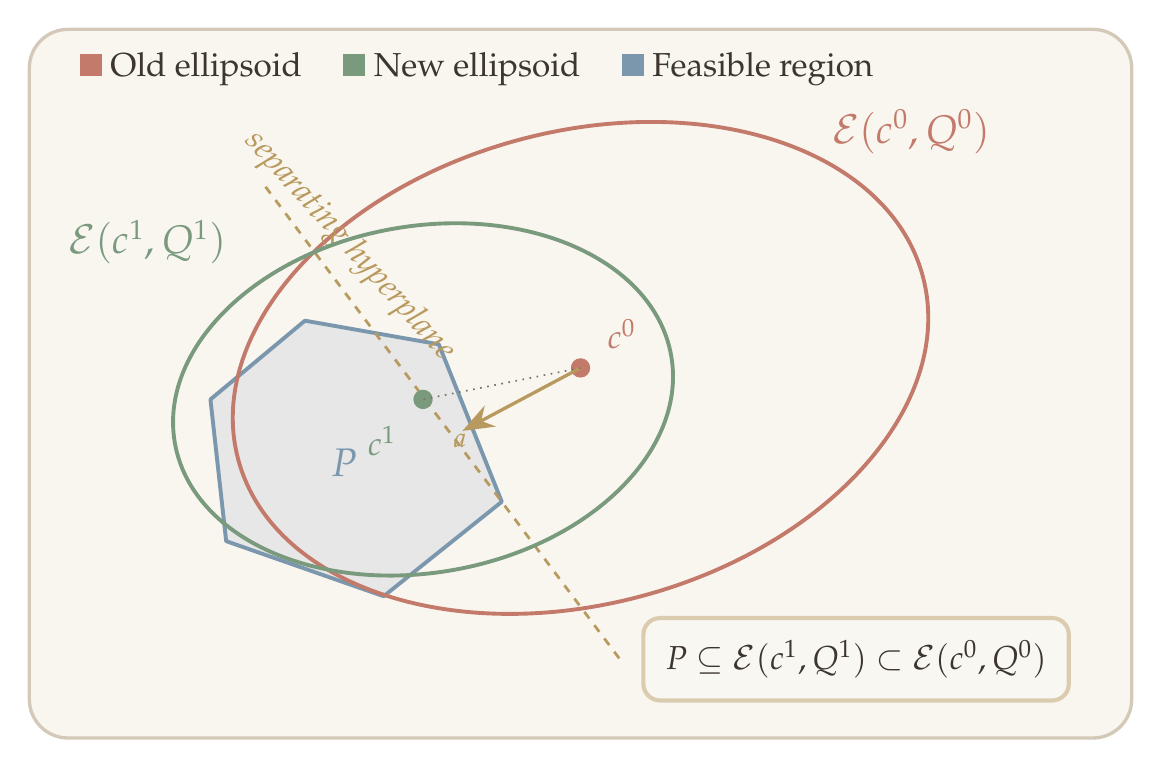
\begin{tikzpicture}[
    >={Stealth[length=4mm, width=3mm]},
    every node/.style={text=dkbrown},
    line width=1.5pt,
  ]

  % Background
  \fill[cream, rounded corners=14pt] (-2.0,-1.5) rectangle (12.0,7.5);
  \draw[border, line width=1.2pt, rounded corners=14pt] (-2.0,-1.5) rectangle (12.0,7.5);

  % === Feasible polytope P (blue filled) ===
  \fill[stblue, opacity=0.15]
    (0.5,1.0) -- (2.5,0.3) -- (4.0,1.5) -- (3.2,3.5) -- (1.5,3.8) -- (0.3,2.8) -- cycle;
  \draw[stblue, line width=1.4pt, line join=round]
    (0.5,1.0) -- (2.5,0.3) -- (4.0,1.5) -- (3.2,3.5) -- (1.5,3.8) -- (0.3,2.8) -- cycle;
  \node[font=\Large\bfseries, text=stblue] at (2.0,2.0) {$P$};

  % === Original ellipsoid E(c^0, Q^0) (terracotta) ===
  \draw[terracotta, line width=1.4pt, rotate around={15:(5.0,3.2)}]
    (5.0,3.2) ellipse (4.5cm and 3.0cm);
  \node[font=\Large\bfseries, text=terracotta] at (9.2,6.2)
    {$\mathcal{E}(c^0, Q^0)$};

  % Center c^0
  \fill[terracotta] (5.0,3.2) circle (3.5pt);
  \node[font=\large, text=terracotta, anchor=south west] at (5.2,3.3) {$c^0$};

  % === Separating hyperplane (dashed rwgold) ===
  % Oriented so P is on one side, c^0 is on the other
  \draw[rwgold, line width=1.0pt, dashed]
    (1.0,5.5) -- (5.5,-0.5);
  \node[font=\large\itshape, text=rwgold, rotate=-48, anchor=south] at (1.8,4.5)
    {separating hyperplane};

  % Arrow from c^0 in the direction of the hyperplane normal (toward P)
  \draw[rwgold, ->, line width=1.2pt]
    (5.0,3.2) -- (3.5,2.4);
  \node[font=\normalsize, text=rwgold, anchor=north east] at (3.7,2.5) {$a$};

  % === New ellipsoid E(c^1, Q^1) (sage) ===
  \draw[sage, line width=1.4pt, rotate around={10:(3.0,2.8)}]
    (3.0,2.8) ellipse (3.2cm and 2.2cm);
  \node[font=\Large\bfseries, text=sage] at (-0.5,4.8)
    {$\mathcal{E}(c^1, Q^1)$};

  % Center c^1
  \fill[sage] (3.0,2.8) circle (3.5pt);
  \node[font=\large, text=sage, anchor=north east] at (2.8,2.6) {$c^1$};

  % Dotted path from c^0 to c^1
  \draw[wmgray, line width=0.6pt, dotted] (5.0,3.2) -- (3.0,2.8);

  % Legend
  \node[font=\large, anchor=west, text=dkbrown] at (-1.5,7.0)
    {\textcolor{terracotta}{\rule{8pt}{8pt}} Old ellipsoid
     \quad \textcolor{sage}{\rule{8pt}{8pt}} New ellipsoid
     \quad \textcolor{stblue}{\rule{8pt}{8pt}} Feasible region};

  % Annotation box
  \node[font=\large, text=dkbrown, align=center,
        fill=rwgold!8, draw=rwgold!50, rounded corners=6pt,
        inner sep=8pt] at (8.5,-0.5)
    {$P \subseteq \mathcal{E}(c^1, Q^1) \subset \mathcal{E}(c^0, Q^0)$};

\end{tikzpicture}
\end{document}
